\documentclass[10pt]{beamer}
\usepackage{xeCJK}
\usepackage{graphicx}
\usepackage{booktabs}
\usepackage{listings}
\usepackage{multirow}
\usepackage{mathtools}
\usepackage{ulem}
\usefonttheme[onlymath]{serif}
\usetheme{metropolis}
\setbeamercolor{footnote mark}{fg=blue}% set footnote color in beamer
\setbeamerfont{footnote}{size=\tiny}
\begin{document}
	\title{数学相关选讲}
	\date{\today}
	\author{huhao}
	\maketitle
	\clearpage
	\begin{frame}
		\frametitle{目录}
		\begin{columns}
			\begin{column}{5.5cm}
				
				\begin{itemize}
					\item 数论
					\begin{itemize}
						\item 模意义下乘法群
						\item 积性函数
						\item 不定方程
						\item 高斯整数
						\item 分圆多项式
					\end{itemize}
					\item 线性代数
					\begin{itemize}
						\item 行列式
						\begin{itemize}
							\item 特殊矩阵行列式
							\item LGV引理
						\end{itemize}
						\item 线性空间,线性映射
						\item 特征向量,特征值,对角化
						\item 内积空间
					\end{itemize}
				\end{itemize}
			\end{column}
			\begin{column}{5.5cm}
				\begin{itemize}
					\item 群论
					\begin{itemize}
						\item 群,Abel群,置换群
					\end{itemize}
					\item 其它
					\begin{itemize}
						\item 类欧几里得算法
						\item 纳什均衡
					\end{itemize}
				\end{itemize}
			\end{column}

		\end{columns}

		\sout{常见的就不讲了,都到NOI了估计都会。}
	\end{frame}
	\section{群论}
	\begin{frame}
		\frametitle{定义}
	
		\begin{itemize}
			\item 代数系统$(A,O_1,O_2,\dots,O_m)$:若干元素组成的集合$A$,以及若干元素间的运算$O_i$,满足定义域是$A^k$,值域是$A$。
			\item 半群$(A,\cdot)$:代数系统;$\cdot:A^2\rightarrow A$,且$x(yz)=(xy)z$。
			\item 群的积:$(A,\cdot)\times(B,\cdot)=\{A\times B,\cdot\}$,且$(u,v)\cdot(a,b)=(u\cdot a,v\cdot b)$。
			\item 含幺半群$(A,\cdot)$:半群;$\exists e,xe=x$。可以发现,$ex=x$。
			\item 群$(A,\cdot)$:含幺半群;$\forall x,\exists y,yx=e$。可以证明,只要任意一个元素存在左逆元,那么它就有唯一的逆元。
			\item Abel群$(A,\cdot)$:群;$xy=yx$。 Abel群一个很重要的性质是$a^kb^k=(ab)^k$。
			\item 循环群$(A,\cdot)$:群;$\exists x,\forall y,\exists k,x=y^k$,不难发现,循环群是Abel群。
		\end{itemize}

	\end{frame}
	\begin{frame}
		\frametitle{同构与同态}
	
		若$f:A\rightarrow B$,$(A,\cdot),(B,\cdot)$是代数系统,且$f(a)+f(b)=f(ab)$则称($f$是)$A,B$(的)同态。

		如果$f$是双射,则称为同构。

		容易验证,所有$n$维循环群是模$n$意义下加法群(下面简记为$Z_n$)的同构。

		容易证明,同态与同构会保留上一页中代数系统的性质。
	
	\end{frame}
	\begin{frame}
		\frametitle{生成元}
	
		在群中, 定义$\langle a\rangle =\{x|x=a^k\}$,$O\langle a\rangle =|\langle a\rangle |$称为$a$的阶,若$O\langle x\rangle =|A|$,则称$x$为$A$的生成元。

		不难发现。
		
		\begin{itemize}
			\item $x\in Z_n,O\langle x\rangle |n$。
			\item $O\langle x\rangle =O\langle -x\rangle $。
		\end{itemize}
	\end{frame}
	\begin{frame}
		\frametitle{Abel群的性质}
	
		\textbf{所有有限Abel群$(A,\cdot)$与$Z_{i_1}\times Z_{i_2}\times \dots Z_{i_n}$(若干循环群的积)同构。}
		
		记$|A|=n$,取$O\langle x\rangle $最大的$x$,则$\langle x\rangle $构成子群,且可以找出$n/O\langle x\rangle $个大小为$O\langle x\rangle $集合,使得集合中所有元素乘上$\langle x\rangle $中的元素依然在这个集合中(这可以不断找一个元素$u$,然后生成集合$\{u^k\}$,这样不同集合肯定是不交的)。

		若$O\langle x\rangle \not=n$,则有多个集合,若将这些集合间的乘运算规定为各取一个元素相乘,得到的结果在的集合。则这些集合和乘法也构成群$(B,\cdot)$。

		假如$(B,\cdot)$与$C=Z_{i_1}\times Z_{i_2}\times \dots Z_{i_n}$同构,若能证明$A$与$C\times Z_{O\langle x\rangle }$同构,则可根据归纳法证明。

		不妨把$B$中的元素(一个集合),通过同构的函数映射至$C$中的元素,通过$(j_1,j_2,\dots j_n),0\le j_k<i_k$表示。
	\end{frame}
	\begin{frame}
		\frametitle{续}
	
		对于群乘积的每一维$Z_{i_k}$,可以在$(0,0,\dots,1,\dots 0)$对应集合$t_k$中(第$k$位为$1$)(暂时)任取一个元素$u_k$作为这个群的代表,假定$u_k^{i_k}=e_A$(否则下面将在$t_k$中找到一个代替这个$u_k$的元素),因为后续证明需要用到这一点。

		如果$u_k^{i_k}\not=e_A$,那么有$u_k^{i_k}=x^y$,则(下式用到了$u_k^r=e_A\Rightarrow i_k|r$,这个可以是根据$t_k$的定义得到的):
		
		$$
			O\langle u_kx^l\rangle =i_k\dfrac{O\langle x\rangle }{(y+li_k,O\langle x\rangle )}
		$$

		根据$x$的定义,有:$i_k\le(y+li_k,O\langle x\rangle )$

		取$l=\lfloor\dfrac{y}{i_k}\rfloor$即可得到$i_k|y$。

		则$u_k'=u_kx^{-\frac y{i_k}}$满足$u_k'^{i_k}=e_A$,用$u_k'$代替任取的$u_k$即可。
	
	\end{frame}
	\begin{frame}
		\frametitle{续}
	
		对于集合$(j_1,\dots j_n)$,不妨用$r_{j_1,\dots j_n}=\prod_{k}u_k^{j_k}$代表(根据定义,则个元素一定在集合内)。

		所以$(\{r\},\cdot)$对运算封闭,它是一个群。可以将$A$中的元素表示为$(u,v),u\in \{r\},v\in \langle x\rangle $,这样可以唯一的表示出$|A|=|\{r\}|O\langle x\rangle $个元素,如果将这样的一一对应关系记为函数$f$,则$f$是$(A,\cdot)$与$(\{r\},\cdot)\times(\langle x\rangle ,\cdot)$的同构。

		所以$A$与$C\times Z_{O\langle x\rangle }$同构(这里没有证明$\{r\}$与$C$同构,可以尝试自行证明。同时可以发现此部分可以不证明,因为已经可以归纳地找到与$r$同构的若干循环群的积了),证明完毕。
	
	\end{frame}
	\begin{frame}
		\frametitle{续}
	
		更进一步,我们知道了$A$与$\prod_j Z_{i_j}$同构,则有:$|Z_{i_j}|~{\big|}~|A|$。

		则对于$A$中的元素$x$,通过同构映射至$\prod_j Z_{i_j}$中的元素$(x_1\dots x_k)$,则$x^{|A|}$可以映射至$(x_1\dots x_k)^{|A|}=(x_1^{|A|}\dots x_k^{|A|})=(e_1\dots e_k)$,即$x^{|A|}=e$。
	
	\end{frame}
	\begin{frame}
		\frametitle{将Abel群分解为循环群}
	
		和证明中的构造方式一致:

		不妨记要分解的Abel群为$A$,遍历$A$中元素,找到$O\langle x\rangle$最大的$x$,提出所有$x^k$。

		然后将$A$划分为$\dfrac{|A|}{O\langle x\rangle}$个集合,递归的将这些集合划分为循环群。

		然后找出每个集合的代表元,这些代表元组成集合$B$,就将$A$划分为了$B\times \langle x\rangle$,$B$划分为循环群方式在上一步已经计算出来了。

		这样每一次都会使要划分为循环群的元素个数除以$2$,这样就可以$O(n\log n)$的时间复杂度内划分开。
	
	\end{frame}
	\begin{frame}
		\frametitle{循环群性质}
	
		\textbf{$Z_{xy}$与$Z_x\times Z_y$同构,其中$(x,y)=1$}。
		
		如果令$1_A$为$A$的生成元,则:

		\begin{itemize}
			\item $1_{xy}=(1_x,1_y)$
			\item $(1_x,1_y)=(1_{xy}^y,1_{xy}^x)$
		\end{itemize}

		上面分别给出了双向的构造。

		\textbf{循环群$Z_n$生成元个数为$\varphi(n)$。}

		考虑一个生成元$g$,则可以将其它元素写成$g^k$的形式,$O\langle g^k\rangle=\dfrac{n}{(n,k)}$,则满足$(n,k)=1$的$g^k$是生成元,则一共是$\varphi(n)$个。
	
	\end{frame}
	\section{数论}
	\begin{frame}
		\frametitle{模意义下乘法(半)群}
	
		对于模$n$意义下的乘法半群,如果仅考虑$Z_n^*=\{x|(n,x)=1\}$,那么这就是一个Able群(可以通过裴蜀定理证明),可以用$\varphi(n)$来表示出它的元素个数。

		由Abel群的性质可知:$(n,x)=1\Rightarrow x^{\varphi(n)}=1$。
	
	\end{frame}
	\begin{frame}
		\frametitle{$Z_p^*$}
	
		对于奇质数$p$,$Z_p^*=([1,p-1],\times)$是Abel群。在这个群中,$f(x)=a_nx^n+\dots+a_0=0$的解的个数不超过$n$:

		若$x_n$是方程的解,那么$f(x)=(x-x_n)g(x)$,而$g(x)$最多有$n-1$个解不在这$1+(n-1)$个解中的元素$y$这会使$(y-x_n)$和$g(y)$都不是$0$。

		根据这个定理(拉格朗日定理),可以证明上述群是循环群:

		根据Abel群与若干循环群之积同构,可以得到:对于任意$x\in[1,p-1]$,有$O\langle x\rangle|p-1$,因为$O\langle x\rangle$等于在每一个循环群上阶的最小公倍数。

		所以不妨令$S_d=\{x|O\langle x\rangle=d\}$,于是若$d$不是$p-1$的约数,一定有$S_d=\emptyset$。

		又如果{\color{red}有}$O\langle x\rangle=d$,那么$x^{k}=1$就是$x^d=1$的解,根据拉格朗日定理,这$d$个数就是唯$d$解,如果$(k,d)=1$,那么$O\langle x^k\rangle=d$,即$|S_d|=\varphi(d)$。
	
	\end{frame}
	\begin{frame}
		\frametitle{续}
	
		于是有$S_d=0$或$S_d=\varphi(d)$(前者是上一页中把红色的字换成“没有”的情况),又有:

		$$
		p-1=\sum_i |S_i|\le \sum_{d|p-1} \varphi(d)=p-1
		$$

		所以$|S_d|=\varphi(d)[d|p-1]$。所以$S_{p-1}\not=\emptyset$,于是就证明了上面讨论的群是循环群。称原根为满足$O\langle x\rangle=p-1$的$x$,即这个群的生成元。
	
	\end{frame}
	\begin{frame}
		\frametitle{$Z^*_{p^2}$}
	
		不妨再看看模$p^2$下的情况,现在我们要证明的是存在$x\in Z^*_{p^2},O\langle x\rangle=(p-1)p=\varphi(p^2)$。

		不妨考虑$p$的原根$g$,对于$g+ip,i\in Z^+$,有:$\varphi(p)|O\langle g+ip\rangle,O\langle g+ip\rangle|\varphi(p^2)$,所以$O\langle g+ip\rangle\in\{\varphi(p),\varphi(p^2)\}$。

		假如$Z_{p^2}^*$不是循环群,则$O\langle g\rangle=O\langle g+p\rangle=\varphi(p)$,则:

		$$
		\begin{aligned}
			&1=(g+p)^{\phi(p)}=\sum_{i=0}^{p-1}{p-1\choose i}p^{i}g^{p-1-i}=\\
			&1+g^{-1}p(p-1)+0+\dots+0=1-g^{-1}p
		\end{aligned}
		$$

		则$p|g^{-1}$,矛盾,所以$g,g+p$一定有一个阶为$\varphi(p^2)$。
	
	\end{frame}
	\begin{frame}
		\frametitle{$Z^*_{p^c}$}
	
		考虑$g$为$Z^*_{p^2}$的原根,则可以通过归纳法:假设$g$为$Z^*_{p^{c-1}}$的原根,则在$Z^*_{p^c}$中有$O\langle g\rangle\in\{\varphi(p^{c-1}),\varphi(p^c)\}$,不妨设:

		$$
		g^{\varphi(p^{c-2})}=g^{(p-1)p^{c-3}}=1+p^{c-2}k\not=1
		$$

		则:

		$$
		g^{\varphi(p^{c-1})}=(1+p^{c-2}k)^p=1+p^{c-1}k
		$$

		由于$k\not=0$,也就是说$g^{\varphi(p^{c-1})}\not=1$,所以$O\langle g\rangle=\varphi(p^c)$
	
	\end{frame}
	\begin{frame}
		\frametitle{$Z^*_{2p^c}$}
	
		类似的,考虑一下$Z^*_{2p^c}$,不难证明:$f(x)=x\bmod p^c$是$Z^*_{2p^c}$到$Z^*_{p^c}$的同构映射,所以它的性质和$Z^*_{p^c}$一样。
	
	\end{frame}
	\begin{frame}
		\frametitle{总结}
	
		对于奇质数$p$,$Z^*_{p^c},Z^*_{2p^c}$都是循环群,即有原根,且恰有$\varphi(\varphi(p^c))$个。

		不难验证,$Z^*_2,Z^*_4$都有原根,分别是$1;1,3$。

		上述群中元素可以用一个正整数来代表,乘法操作就可以变为$Z_{\varphi(p^c)}$上的加操作。

		对于其它的整数$n$,$Z^*_n$是Abel群,可以划分为若干循环群之积。群中元素可以用一个数组代表,乘法操作也可以变为若干循环群积上的加操作。
	
	\end{frame}
	\begin{frame}
		\frametitle{例}
	
		给定$n,a,b$,满足$n\le 10^6,(b,n)=1$,求下式解的个数:

		$$
		x^a \bmod n=b
		$$

		加强版:没有$(b,n)=1$的限制。
	
	\end{frame}
	\begin{frame}
		\frametitle{例}
	
		给定质数$n$,求有多少组$(x,y)$,满足:

		\begin{itemize}
			\item $1\le x,y\le (n-1)n$
			\item $x^y\equiv y^x\mod n$
		\end{itemize}

		思考题:$n$不一定是质数,$x,y\le \varphi(n)n$
	
	\end{frame}
	\begin{frame}
		\frametitle{积性函数}
	
		如果对于互质的$u,v$,有$f(u)f(v)=f(uv)$,那么称$f$为积性函数。

		狄利克雷卷积:

		$$
		(f*g)(n)=\sum_{i|n}f(i)g(\dfrac ni)
		$$

		莫比乌斯反演:

		$$
		f=1*F\Rightarrow F=\mu*f
		$$

		当然,有时使用下面这个变形会简单些:

		$$
		[n=1]=\sum_{d|n}\mu(d)
		$$
	
	\end{frame}
	\begin{frame}
		\frametitle{杜教筛}
	
		你知道$\sum (f*g)(n),\sum f(n),\forall n\in Z^+$,需要求出$\sum g(n)$。

		$$
		\sum_{i=1}^n (f*g)(i)=\sum_{1\le ij\le n}f(i)g(j)=f(1){\color{red}\sum_{j=1}^n g(j)}+\sum_{i=2}^n f(i)\sum_{j=1}^{\lfloor\frac{n}{i}\rfloor} g(j)
		$$

		可以发现,只要知道$\sum_{n=1}^{m}(f*g)(n),\sum_{n=1}^{m} f(n)$,所有$m\le N^{\frac 23},m=\dfrac Nd$时的取值,就可以在$O(N^{\frac 23})/O(N^{\frac 23}\log n)$的时间复杂度内求出$\sum_{n=1}^mg(n)$的取值($m$范围与前文相同)。

		值得注意的是,这里没有用到积性函数的性质,所以本页所有函数均不要求积性函数。
	
	\end{frame}
	\begin{frame}
		\frametitle{续}
	
		更进一步的,不难发现,上面的过程可以通过$f,g$的若干前缀和,得到$f*g^{-1}$的前缀和。可以通过两步得到$f*g$的若干前缀和:

		$$
		\begin{aligned}
			I,g\rightarrow &g^{-1}\\
			f,g^{-1}\rightarrow &f*g\\
		\end{aligned}
		$$
	
	\end{frame}
	\begin{frame}
		\frametitle{powerful number优化}
	
		假如要求$f*g$的前缀和,其中$f$是积性函数且若存在次数为$1$质因子则取值为$0$(其它的数则称为powerful number),$g$的前缀和要能快速求出(只需要用到$\dfrac Nd$的值,但采用杜教筛的话会成为瓶颈)。

		这时可以利用:

		$$
		\sum_{i=1}^n (f*g)(i)=\sum_{i=1}^n f(i)\sum_{j=1}^{\frac ni}g(j)
		$$

		因为$f$只有$O(\sqrt n)$处有值,所以能$O(1)$求出$g$的前缀和的话复杂度就是$O(\sqrt n)$的。

		同样的,$f$只有$O(\sqrt n)$种不同的前缀和,所以也可以利用杜教筛求解。
		
	\end{frame}
	\begin{frame}
		\frametitle{复杂度证明}
	
		不难发现,只有形如$a^2b^3$的数才是powerful number,所以可以用下式确定上界:

		$$
		\sum_{i,j}[i^2j^3\le n]
		$$

		利用积分来逼近:

		$$
		\int_{0}^{\sqrt n} \sqrt[3]{\dfrac n{x^2}}\mathrm dx=O(\sqrt n)
		$$
	
	\end{frame}
	\begin{frame}
		\frametitle{应用}
	
		不难发现,如果$f=g*h$,$g,h$是积性函数,且$h$仅在powerful number处非$0$,那么:

		$$
		f(1)=g(1)h(1)=1,f(p)=g(1)h(p)+h(1)g(p)=g(p)
		$$
		
		也就是说,要求一个积性函数$f$的值,如果存在一个“方便求和”的积性函数$g$,使得对于任意一个质数$p$,有$f(p)=g(p)$,且$f(1)=1$,就可以通过这种方法快速求解。
	
	\end{frame}
	\begin{frame}
		\frametitle{例}

		给定$n$,对积性函数$f$的前$n$项求和,其中$f(p^c)=p\oplus c$。
	
	\end{frame}
	\begin{frame}
		\frametitle{解}
	
		令$g(x)=[x=1]+2[x=2]$,那么$f=g*\varphi*h$,其中$h$仅在powerful number处非0。
	
	\end{frame}
	\begin{frame}
		\frametitle{不定方程}

		形如$a^2+b^2=c^2$就是不定方程,一般来说需要求出所有的整数解。
	
	\end{frame}
	\begin{frame}
		\frametitle{化为参数方程形式}
	
		注意到这是齐次的,可以通过两边同时除以$c^2$来变为求有理数解降维:$u^2+v^2=1$。

		不难发现$u=1$时,$v=0$是唯一解,可以令$u=kv+1$,转为求$v,k$的解。

		现在就变成了求$k^2v^2+2kv+v^2=0$的解,剔除$v=0$就是$(k^2+1)v+2k=0,v=\dfrac{-2k}{k^2+1}$,就得到了参数方程形式的解!
	
	\end{frame}
	\begin{frame}
		\frametitle{例:projeteuler785}
	
		$$15  (x^2 + y^2 + z^2) = 34  (xy + yz + zx)$$
	
	\end{frame}
	\begin{frame}
		\frametitle{枚举因数}
	
		求最小的可以表示为$100$组两个五边形数的和的五边形数。

		$$
		\dfrac{1}{2}a(3a-1)=\dfrac{1}{2}b(3b-1)+\dfrac{1}{2}c(3c-1)
		$$

		这可以通过枚举$c(3c-1)$的约数求解:

		$$
		(a-b)(3a+3b-1)=c(3c-1)
		$$

		复杂度未知,但跑得特别快。
	
	\end{frame}
	\begin{frame}
		\frametitle{高斯整数}
	
		定义$\mathbf Z=\{a+bi|a,b\in Z\}$,集合内元素称为高斯整数。

		定义高斯整数间的整除为:$a|b\Leftrightarrow \dfrac ba\in \mathbf Z$。定义单位数为$1,-1,i,-i$。

		可以在$\mathbf Z$上定义素数:类似$Z$上的定义,如果一个高斯整数的因数只有$1$和它本身,以及乘上一个单位数,就称为高斯素数。不妨记高斯素数的集合为$P$。

		定义$\mathbf Z$上带余除法为:$a=bq+r$,其中$q$通过$\dfrac ab$四舍五入取到,则$|r|^2=|tb|^2=|(t_r^2+t_i^2)b^2|\le \dfrac 12|b|^2$。于是$\mathbf Z$上可以进行欧几里得算法,用exgcd可以求出$ax+by=(x,y)$的解。

		若$x|yz,x\in P$那么$x|y$或$x|z$:考虑若$x$不是$y$的因数,那么存在$ax+by=1$,于是$axz+byz=z$,则$x|axz+byz=z$。

		由此可以证明,$\mathbf Z$上也有唯一分解定律,不过任意一项都可能会乘以单位数。
	\end{frame}
	\begin{frame}
		\frametitle{高斯素数}
	
		如果$x\in P$,那么一定有$\overline x\in P$,证明:
			
		反证(或者归纳),如果不满足,那么一定有范数最小的$x$。

		若$\overline x=x_1x_2$,那么$x=\overline x_1\overline x_2$与$x\in P$矛盾。

		$ $

		如果$|x|^2$是质数,那么$x\in P$,证明:

		若$x=yz$,那么$|x^2|=|y|^2|z|^2$,那么$y,z$中必有一个是单位数。

	\end{frame}
	\begin{frame}
		\frametitle{续}
	
		现在考虑证明找出高斯素数的分布,不妨考虑一个素数$p$会证明被分解:

		\begin{itemize}
			\item $p=2=(1+i)(1-i)$。
			\item $p\bmod 4=3$,那么$|p|^2=p^2$,若$p\not\in P$则$p=xy$,则$|x|^2|y|^2=p^2$,则$|x|^2=|y|^2=p$,又由于两数平方和不可能$\bmod 4=3$,所以$p\in P$。
			\item $p\bmod 4=1$,则$p$是两个互为共轭的高斯素数的乘积,存在性将在下一页证明,唯一性由唯一分解定律保证。
		\end{itemize}
	\end{frame}
	\begin{frame}
		\frametitle{续}
	
		对于$p\bmod 4=1$的质数$p$,令$t=\dfrac{p-1}2$,则:

		$$
		\prod_{i=1}^t i \bmod p=\prod_{i=1}^t -i \bmod p=s
		$$

		则

		$$
		s^2 \bmod p=\prod_{i=1}^{t}i(p-i) \bmod p=\prod_{i=1}^{p-1} i \bmod p=p-1
		$$

		若$p\in Z$,则由$p|s^2+1$可知$p|s+i$或$p|s-i$,而两者均不可能($i$除不尽)。

		所以$p$不是高斯质数,考虑到$|p|^2=|xy|^2=p^2$,所以$|x|^2=|y|^2=p$,则$y=\overline x$。
	
	\end{frame}
	\begin{frame}
		\frametitle{例}

		有多少范数平方小于$n$的高斯整数没有非单位高斯整数的平方作为因子。
	
	\end{frame}
	\begin{frame}
		\frametitle{分圆多项式}
	
		称以下多项式为分圆多项式
		
		$$
		\Phi_n(x)=\prod_{(i,n)=1}(x-\omega_n^i)
		$$

		它给出了一个重要的多项式的因式分解:

		$$
		\prod_i (x-\omega_n^i)=x^n-1
		$$
	
	\end{frame}
	\begin{frame}
		\frametitle{续}
	
		现在来考察分圆多项式的性质:
		
		$$
		\prod_{i|n}\Phi_i(x)=x^n-1
		$$

		证明可以考虑每一个$(x-\omega_n^k)$被乘在了哪里。

		$ $

		分圆多项式系数都是整数。证明:
		
		归纳证明,假如对于$i<n,\Phi_i(x)\in Z[x]$,则$\Phi_n(x)=(x^n-1)\prod_{i<n,(i,n)=1}\Phi_i(x)$一定是整系数多项式。
	
	\end{frame}
	\begin{frame}
		\frametitle{续}
	
		分圆多项式不是任意两个整系数多项式的乘积。

		这个证明过于繁琐(和前文关于阿贝尔群的证明一样),同时前置知识较难(需要用到高等代数),本文忽略证明。

	\end{frame}
	\begin{frame}
		\frametitle{例}
	
		求所有的能整除$x^n-1$的首项为$1$的整系数多项式的和,并输出带入$x=2$后的值,$n\le 10^7$。
	
	\end{frame}
	\begin{frame}
		\frametitle{例}
	
		给定质数$n$,求有多少个由$1\sim n^2$组成的$n\times n$矩阵,可以通过若干次给某行或某列加减同一个数变为全$0$矩阵。
	
	\end{frame}
	\begin{frame}
		\frametitle{解}
	
		先全部减去一个$1$,然后考虑第$i$行减了$a_i$,第$j$列减了$b_j$,则有:

		$$
		\sum_{i}x^{a_i}\sum_{i}x^{b_i}=\sum_{i=0}^{n^2-1} x^i=\dfrac{x^{n^2}-1}{x-1}=\dfrac{\Phi_1(x)\Phi_n(x)\Phi_{n^2}(x)}{x-1}=\Phi_n(x)\Phi_{n^2}(x)
		$$

		不难发现,$\Phi_{n}=\sum_{i=0}^{n-1}x^{i},\Phi_{n^2}=\sum_{i=0}^{n-1}x^{ni}$都恰有$n$个系数为$1$的,所以$\sum_i x^{a_i}\Phi_n(x)$或是$\sum_i x^{a_i}\Phi_{n^2}(x)$,且$a$可以是任意一个排列,$b$同理,则一共有:

		$2(n!)^2$种方案。
	
	\end{frame}
	\section{线性代数}
	\begin{frame}
		\frametitle{行列式}
	
		\sout{在OI中,行列式可以和其它线代知识分开考虑。}

		行列式的定义:

		$$
		\sum_{p}\mathrm{sgn}(p)\prod_i a_{i,p_i}
		$$

		性质有:

		\begin{itemize}
			\item 某一行/列,加上令一行/列的若干倍,值不变。
			\item 交换两行/两列,值取相反数。
			\item 行列式的值等于下面两式的和:
			\begin{itemize}
				\item 将第一行第一个元素变为$0$后矩阵的行列式。
				\item 将第一行第一列删去后矩阵行列式乘以第一行第一个元素。
			\end{itemize}
		\end{itemize}

		于是,可以解决:
	
	\end{frame}
	\begin{frame}
		\frametitle{例:300iq contest 2D}
	
		\url{https://codeforces.com/gym/102331/problem/D}
	
	\end{frame}
	\begin{frame}
		\frametitle{特殊行列式}
	
		范德蒙德行列式:$a_{i,j}=\hat a_i^j$:$\prod_{i<j}(a_j-a_i)$

		循环矩阵行列式:$a_{i,j}=\hat a_{(i+j)\bmod n}$:$\prod_i f(\omega^i),f(x)=\sum_i \hat a_ix^i$
	
	\end{frame}
	\begin{frame}
		\frametitle{LGV引理}
	
		求两个集合$A,B$间有多少组$n$条两两不相交的路径$A_i\rightarrow B_i$,可以用:

		$$
		\det |c(A_i,B_j)|
		$$

		其中$c(A_i,B_j)$表示从$A_i$到$B_j$的路径数。
	
	\end{frame}
	\begin{frame}
		\frametitle{线性空间}
	
		如果某一个集合$A$,满足$x\in A,y\in A\rightarrow x+y\in A$和$x\in A\rightarrow \lambda x\in A,\lambda\in R$,就称$A$为线性空间,接下来的线性代数部分全在线性空间上讨论。

		称一组元素$\{x_k\}$的张成为:$\mathrm{span}(\{x_k\})=\{y|y=\sum_i \lambda_ix_i,\lambda_k\in R\}$。

		称一组元素$x_k$线性无关,当且仅当$\sum_i \lambda_ix_i=0\Rightarrow \lambda=0$。

		如果$x_1,x_2\dots$为$A$的一个张成,且$x$线性无关,则称它们为$A$的一组基。

		不难发现,如果$A$有一组元素$x_1,\dots x_n$作为基,且元素个数是有限的,则称$A$是有限维的,称$\dim A=n$。

		称两个线性空间的直和$A\oplus B$为$\{u+v|u\in A,v\in B\}$,且要求$w\in A\oplus B$则有唯一的$u\in A,v\in B$使得$w=u+v$。

		如果$U=A\oplus B$,且$u+v=w\in U,u\in A,v\in B$,则称$P_{U,A}w=u,P_{U,B}w=v$为一个投影。
	
	\end{frame}
	\begin{frame}
		\frametitle{线性映射}
	
		定义$L:A\rightarrow B$为线性映射,当且仅当$A,B$为线性空间,且$L(u+v)=L(u)+L(v),L(\lambda u)=\lambda L(u)$。

		如果线性空间$A,B$是有限维的,若$a,b$分别是它们的基,可以将$L$写成矩阵的形式:$\dim A\times \dim B$的矩阵,第$i$列第$j$行的值为$L_{i,j}$,则代表着$L(a_i)=\sum_j L_{i,j}b_j$。

		一般来说,矩阵需要写为:$M(L,a,b)$,即线性变换和它们的基底,如果$a,b$是明确的,或是在讨论中未曾变过,则可以简写为$M(L)$。简单起见,下文有关矩阵操作的$L$均表示$M(L)$。
	
	\end{frame}
	\begin{frame}
		\frametitle{特征值与特征向量,对角化}
	
		如果$L:A\rightarrow A$的线性映射,则称$L$是$A$上的算子。

		不妨重点关注满足$B=L(B),B\subset A$的$B$,称这样的$B$为$L$的不动子空间。

		不妨重点关注$1$维的不动子空间,称这个线性空间中的元素为特征向量,如果$Lv=\lambda v$,那么称$\lambda$为特征值。不难发现,特征向量可以有无穷多个,但特征值最多只有$\dim A$个。下式给出了特征向量及对应的特征值的关系:

		$$
		Lv=\lambda v,(L-\lambda)v=0,\det(L-\lambda I)=0
		$$
	\end{frame}
	\begin{frame}
		\frametitle{对角化}

		如果$L$有$\dim A$个线性无关的特征向量$v_1\dots v_n$,那么$A$可以选取这些元素作为基,又$L(v_i)=\lambda_i v_i$,所以这组基对应矩阵只有对角线上元素非$0$,称这样的矩阵为对角矩阵。

		对于$x=\sum_i a_iv_i$,有:$L^k(x)=\sum_i a_iv_i\lambda_i^k$,这远远比在任取的基下的矩阵乘法简单。所以选取合适的基,使得矩阵对角化是一个优秀的方法。(但是通常来说,求出特征向量不简单)

		更简单的,可以考虑一个每行都是$L$的一个特征向量的矩阵$X$,考虑下式:

		$$
		X^{-1}LX
		$$

		对于$M(L)$的基底$l_i$,有:

		$$
		X^{-1}LXl_i=X^{-1}Lv_i=X^{-1}(\lambda_iv_i)=\lambda_il_i
		$$

	\end{frame}
	\begin{frame}
		\frametitle{内积空间}
	
		在线性空间$V$中,定义内积$\langle x,y\rangle $其中$x,y\in V$,则它满足以下性质:

		\begin{itemize}
			\item 双线性:$L_1(x)=\langle x,y\rangle $和$L_2(y)=\langle x,y\rangle $都是线性映射。
			\item 正定:$\langle x,x\rangle\ge 0$,取等条件为$x=0$。
			\item 共轭对称:$\langle x,y\rangle=\overline{\langle y,x\rangle}$,在$R$中讨论则无需共轭。
		\end{itemize}

		定义$x,y$是正交的,当且仅当$\langle x,y\rangle=0$。

		定义范数$||x||=\langle x,x\rangle^{\frac 12}$。

		如果一组基$v_i$是彼此正交的,那么就有一个简单的办法计算范数(本页下文$x_i=P_{V,v_i} x$即在$v_i$上的投影):

		$$
		||x||^2=\langle x,x\rangle=\langle \sum_i x_iv_i,\sum_i x_iv_i\rangle=\sum_{i,j}x_ix_j\langle v_i,v_j\rangle=\sum_i x_i^2 ||v_i||^2
		$$

		如果每一个$v_i$都是单位向量,即$||v_i||=1$,那么$||x||^2=\sum_i x_i^2$。(即勾股定理)
	
	\end{frame}
	\begin{frame}
		\frametitle{规范正交基}
	
		如上页所述,基底$e_i$是单位的,且是两两正交的,会给使用带来极大的便利,称这一组基底为规范正交基。它还有以下性质(可以通过带入$e_1=(1,0),e_2=(0,1)$理解):

		$$
		x=\sum_i \langle x,e_i\rangle e_i
		$$

		如果一个线性空间有基底$v_i$,那么它一定有规范正交基:

		依次对$i\in[1,n]$执行:

		取$e_i=\dfrac{v_i-\sum_{j<i}\langle v_i,e_j\rangle e_j}{||v_i-\sum_{j<i}\langle v_i,e_j\rangle e_j||}$。

		不难证明这还是一组基底,且两两正交,且都是单位的。
	
	\end{frame}
	\begin{frame}
		\frametitle{正交投影}
	
		对于任一元素$v$,以及线性空间$U$,和它的一组规范正交基$e$,令:

		$$
		P_Uv=\langle v_i,e_i\rangle e_i
		$$

		称为$v$在$U$上的正交投影(和前文定义的类似,如果$W=U\oplus V,v\in V$,且$\forall x\in U,y\in V,\langle x,y\rangle=0$,那么$P_{W,U}v=P_u v$),它有如下性质:

		$$
		\langle P_U,v\rangle=\min_{u\in U}\langle u,v\rangle
		$$

		这类似于"点到直线/平面/超平面最短的距离等于垂线长度"。
		
		当然这里是在$R$上讨论的,因为没有在$C$上定义偏序关系。
	
	\end{frame}
	\begin{frame}
		\frametitle{例}
	
		{\color{red}上式给在线性空间中求距离(范数)最小值带来了很大的便利},比如:

		定义两函数在$[l,r]$上的平方距离为:

		$$
		||f-g||=\int_l^r ||f(x)-g(x)||^2\mathrm dx
		$$

		于是可以取内积为下式来使得范数为上式:

		$$
		\langle f,g\rangle=\int_l^r f(x)g(x)\mathrm dx
		$$

		如果要在$5$次实多项式中找出与$\sin x$在$[-\pi,\pi]$上平方距离最近的,利用上文的方法,可以得到答案$f(x)$:

		$$
		f(x)\approx 0.987862x-0.155271x^3+0.00564312x^5
		$$
	
	\end{frame}
	\begin{frame}
		\frametitle{续}
	
		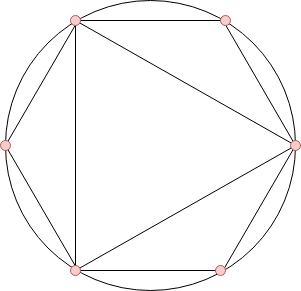
\includegraphics[width=10.5cm]{1.png}
	
	\end{frame}
	\begin{frame}
		\frametitle{例}
		
		给定矩阵$A$和向量$y$,求向量$x$使得下式取最小值:

		$$
		||Ax-y||
		$$
	
	\end{frame}
	\section{其它}
	\begin{frame}
		\frametitle{类欧几里得算法}
	
		求:

		$$
		\sum_i f(x)g(\lfloor\frac{ax+b}c\rfloor)
		$$

		一般来说思路是枚举$y=\lfloor\frac{ax+b}c\rfloor$,然后对满足条件的$x$求和。

		这样就会将的$a,c$的位置对调,如果能将分子里大于等于$c$的部分提到外面就可以变为类似欧几里得算法的复杂度:

		$$
		(a,c)\rightarrow(a\bmod c,c)\rightarrow(c,a\bmod c)\rightarrow(c\bmod(a\bmod c),a\bmod c)\rightarrow \cdots
		$$
	
	\end{frame}
	\begin{frame}
		\frametitle{续}
	
		当然,也有一种更加通用的办法:

		考虑直线$y=\dfrac{ax}b$,依次考虑它和$x=z,y=z,z\in N$的交点,并记录两个整数$\hat x,\hat y$,初始为$0$:

		\begin{enumerate}
			\item 和$x=z,z\in N$相交:给$\hat x$加一,给答案加上$f(\hat x)g(\hat y)$。
			\item 和$y=z,z\in N$相交:给$\hat y$加一。
		\end{enumerate}
	
		然后从$(a,b)=(1,1)$开始,也就是操作为:$(21)^{\infty}$。

		如果$b\leftarrow b+ak$,那么就会$2\leftarrow 1^k2$,例如$(a,b)=(1,3)$就是$(1121)^{\infty}$。

		如果$a\leftarrow a+bk$,那么就会$1\leftarrow 2^k1$,例如$(a,b)=(7,3)$就是$(2212212221)^{\infty}$。
	\end{frame}
	\begin{frame}
		\frametitle{续}
	
		然后从就可以得到一棵树,记录了每一个元素是怎么一步步得到最终元素的。

		每一层中,$0$所衍生出的所有子树和$1$所衍生出的所有子树分别同构,那么就只要知道如下信息就可以很好的完成此题:

		\begin{itemize}
			\item $0$和$1$所衍生出的子树分别会给后面的子树带来的影响$e$。
			\item 前面子树带来的影响为$e$时,$0$和$1$所衍生出的子树的具体情况。
		\end{itemize}

		注意到如果某一层时$u\leftarrow v^ku$,那么可以划分为$u\leftarrow v^{\frac k2}v^{\frac k2}u$,在这里进行“快速幂”可以简化分析。

		注意到有时操作区间并不是像理想中的那样恰好覆盖一颗完整的树(比如$i$上界不是$c$的倍数,或是$b$不为$0$),此时可以像线段树一样查询。具体的:开始位置可以考虑第一次$(ai+b)\bmod c<(a,c)$(如果$a,c$互质就是$c|ai+b$)的$i$,这是一个整点,往前$i$个$1$就是开始的位置;结束位置就是开始位置往后$\lfloor\dfrac{a(n-1)+b}c\rfloor$个$1$。

		由于这样查询比较复杂,所以尽量使用我所介绍的第一种方法。
	
	\end{frame}
	\begin{frame}
		\frametitle{例:loj6440 万能欧几里得}
	
		$$
		\sum_{i=1}^L A^iB^{\lfloor \frac{ai+b}c\rfloor}
		$$

		其中$a,b,c\in Z$,$A,B$是矩阵。
	
	\end{frame}
	\begin{frame}
		\frametitle{解答}
	
		注意到如果需要将$A^uB^v$变为$A^{u+x}B^{v+y}$,可以通过下式解决:

		$$
		A^x(A^uB^v)B^y=A^{u+x}B^{v+y}
		$$

		再通过记录$(x,y)$就知道做到第二种方法中所需要的信息。
	
	\end{frame}
	\begin{frame}
		\frametitle{纳什均衡}
	
		你和另一个人分别有决策集合$A,B$,你和对方需要给出混合策略$f,g$,满足:

		$$
		\sum_{a\in A} f(a)=\sum_{b\in B} g(b)=1
		$$

		纳什均衡就是对于下式:

		$$
		\sum_{a\in A}\sum_{b\in B}f(a)g(b)v_{A/B}(a,b)
		$$

		无论如何改变$f/g$,$v_{A/B}$的和都不会比现在的大。
	
	\end{frame}
	\begin{frame}
		\frametitle{例}
	
		在下面所表示的收益表下,求纳什均衡:
		\begin{tabular}{|c|c|c|}   
			\hline   $v_A/v_B$ & x & y \\   
			\hline   x & 3/-3 & -2/+2  \\ 
			\hline   y & -2/+2 & 1/-1  \\  
			\hline   
		\end{tabular}

		不难发现:$f(x)=g(x)=\dfrac 38,g(y)=g(y)=\dfrac 58$。
	\end{frame}
	\begin{frame}
		\frametitle{线性规划求解零和纳什均衡}
	
		如果$v_A+v_B=0$,则称此博弈是零和的,所以可以认为第二个人想让第一个人的收益最小。

		即需要求:

		$$
		\max_f \min_g \sum_{i,j} f(i)g(j)v(i,j)
		$$

		可以证明,上式与下式相等,也就是说一定能求出纳什均衡:

		$$
		\min_g \max_f \sum_{i,j} f(i)g(j)v(i,j)
		$$
	
	\end{frame}
	\begin{frame}
		\frametitle{续}
	
		也就是说,要求:

		$$
		\begin{aligned}
			&&&\max V.\\
			\mathrm{st.}&&&\sum_{i} f(i)=1\\
			&&&\sum_{i} f(i)v(i,j)\ge V,j\in B
		\end{aligned}
		$$

		这就是线性规划问题。
	
	\end{frame}
\end{document}